\subsection{Achievements}\label{subsec:achievements}

Im Spiel können durch erreichen von gewissen Merkmalen, z.B. eine gewisse Menge an Geld verdient oder das erste Mal im Gefängnis sein, Achievements freigeschaltet werden. Diese erscheinen bis zum Freischalten nur als Icon mit Fragezeichen im Achievements Menü, nach dem Freischalten mit einem eigenen Bild.
\vspace{0.5cm} 
\begin{center}
    \begin{tabular}{ccccc}
        
\includegraphics[width=1.5cm]{./figures/Question.png} & 
        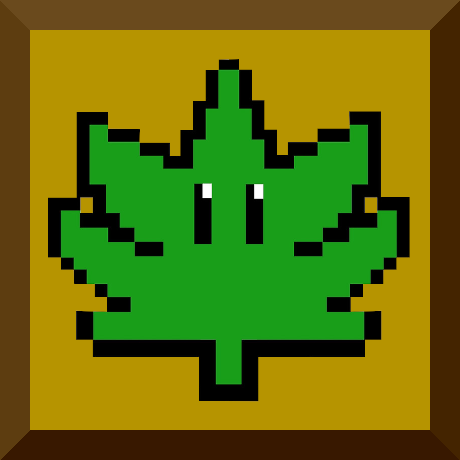
\includegraphics[width=1.5cm]{./figures/Weed.png} & 
        
\includegraphics[width=1.5cm]{./figures/Money.png} & 
        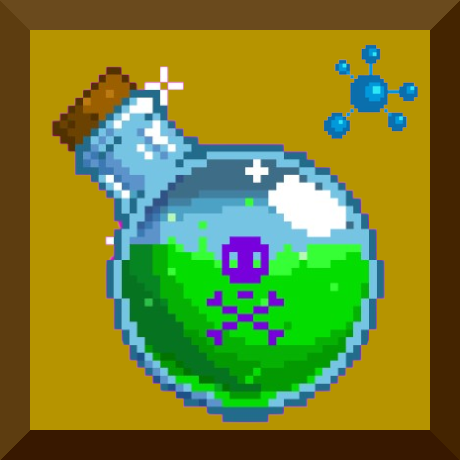
\includegraphics[width=1.5cm]{./figures/Potion.png} & 
        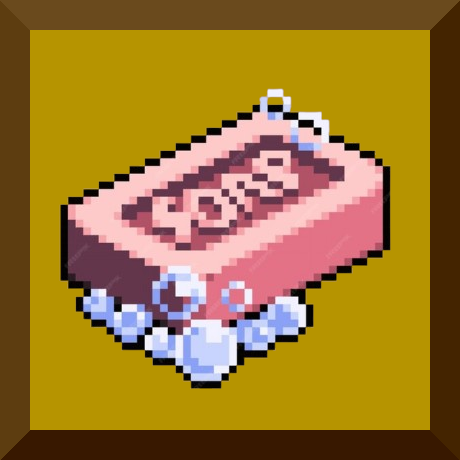
\includegraphics[width=1.5cm]{./figures/Soap.png} \\
    \end{tabular}
\end{center}
\begin{center}
    Abbildung 4: Beispiele für achievement Icons, locked und unlocked.
\end{center}

\vspace{1.5cm} 

\textbf{Zu erreichende Achievements und die Bedingungen zum Freischalten:}
\begin{itemize}
    \item \textbf{New Sprout in Town}: Craft and sell for the first time \newline - Nach dem ersten Verkaufen.
    \item \textbf{We Bankin’}: Make your first Million\$ \newline - Nach erreichen eines Geldbestandes von 1000000 Einheiten.
    \item \textbf{Walter Who?}: Unlock all the recipes \newline - Nach freischalten aller Rezepte.
    \item \textbf{Don’t Drop the Soap}: Land for the first time in jail \newline - Nach der ersten Gefangennahme durch die Polizei.
    \item \textbf{So Blue…}: Deliver 1.000kg of pure meth \newline - Nach dem Herstellen und Verkaufen von 1000 Einheiten Drogen.
    \item \textbf{Scavenger}: Find 10 different ingredients in the map \newline - Nach dem Finden von mindestens 10 verschiedenen Zutaten.
    \item \textbf{Most Wanted}: Reach a 100\% wanted level \newline - Nach dem erreichen eines Wanted Levels von 100\%.
    \item \textbf{Sharp Shooter}: Take down 100 cartel members \newline - Nach dem töten von 100 Cartel NPCs.
    \item \textbf{Chill Spot}: Successfully hide in 10 bushes \newline - Nach dem Verstecken in mindestens 10 Gebüschen.
    \item \textbf{Cancer Free}: Complete the game by finally healing from your cancer \newline - Nach dem Kaufen der heilenden Medizin und Gewinnen des Spiels.
\end{itemize}